%  article.tex (Version 3.3, released 19 January 2008)
%  Article to demonstrate format for SPIE Proceedings
%  Special instructions are included in this file after the
%  symbol %>>>>
%  Numerous commands are commented out, but included to show how
%  to effect various options, e.g., to print page numbers, etc.
%  This LaTeX source file is composed for LaTeX2e.

%  The following commands have been added in the SPIE class 
%  file (spie.cls) and will not be understood in other classes:
%  \supit{}, \authorinfo{}, \skiplinehalf, \keywords{}
%  The bibliography style file is called spiebib.bst, 
%  which replaces the standard style unstr.bst.  

\documentclass[]{spie}  %>>> use for US letter paper
%%\documentclass[a4paper]{spie}  %>>> use this instead for A4 paper
%%\documentclass[nocompress]{spie}  %>>> to avoid compression of citations
%% \addtolength{\voffset}{9mm}   %>>> moves text field down
%% \renewcommand{\baselinestretch}{1.65}   %>>> 1.65 for double spacing, 1.25 for 1.5 spacing 
%  The following command loads a graphics package to include images 
%  in the document. It may be necessary to specify a DVI driver option,
%  e.g., [dvips], but that may be inappropriate for some LaTeX 
%  installations. 
\usepackage[]{graphicx}
\usepackage{url}
\usepackage[table, xcdraw]{xcolor}
\usepackage{subcaption}
\usepackage{amsmath}

\title{3D scanning by means of dual-projector structured light illumination} 

%>>>> The author is responsible for formatting the 
%  author list and their institutions.  Use  \skiplinehalf 
%  to separate author list from addresses and between each address.
%  The correspondence between each author and his/her address
%  can be indicated with a superscript in italics, 
%  which is easily obtained with \supit{}.

\author{Daniel L. Lau\supit{a} and Ying Yu\supit{a}
\skiplinehalf
\supit{a}University of Kentucky, Address, Lexington, US; \\
%\supit{b}University of Kentucky, Address, Lexington, US
}

%>>>> Further information about the authors, other than their 
%  institution and addresses, should be included as a footnote, 
%  which is facilitated by the \authorinfo{} command.

\authorinfo{Further author information: (Send correspondence to A.A.A.)\\A.A.A.: E-mail: aaa@tbk2.edu, Telephone: 1 505 123 1234\\  B.B.A.: E-mail: bba@cmp.com, Telephone: +33 (0)1 98 76 54 32}
%%>>>> when using amstex, you need to use @@ instead of @
 

%%%%%%%%%%%%%%%%%%%%%%%%%%%%%%%%%%%%%%%%%%%%%%%%%%%%%%%%%%%%% 
%>>>> uncomment following for page numbers
% \pagestyle{plain}    
%>>>> uncomment following to start page numbering at 301 
%\setcounter{page}{301} 
 
  \begin{document} 
  \maketitle 

%%%%%%%%%%%%%%%%%%%%%%%%%%%%%%%%%%%%%%%%%%%%%%%%%%%%%%%%%%%%% 
\begin{abstract}
This document shows the desired format and appearance of a manuscript prepared for the Proceedings of the SPIE.  It contains general formatting instructions and hints about how to use LaTeX.  The LaTeX source file that produced this document, {\tt article.tex} (Version 3.3), provides a template, used in conjunction with {\tt spie.cls} (Version 3.3).  
\end{abstract}

%>>>> Include a list of keywords after the abstract 

\keywords{Manuscript format, template, SPIE Proceedings, LaTeX}

%%%%%%%%%%%%%%%%%%%%%%%%%%%%%%%%%%%%%%%%%%%%%%%%%%%%%%%%%%%%%
\section{Introduction}
\label{sec:intro}  % \label{} allows reference to this section
As one of the non-contact 3D shape measurement techniques, the structured light illumination (SLI) has been known for its high resolution and high speed \cite{chen00}. Conventional SLI systems consist of one projector, one camera and one processing unit which is usually a computer. The projector presents patterns that are encoded with some information related to the pixel locations on the object to be measured. If the projection is on a flat surface, the patterns seen should be identical to its original design. However, with the presence of the non-planar object under the projection, what is actually seen from the camera is the distorted patterns on the surface of the object. By comparing and analyzing the distortion in the images taken by the camera, the 3D surface of the object can eventually be reconstructed in a processing unit.

Within the scope of this fundamental idea and system structure, a lot of research has been done over the past several decades \cite{geng11}. Different practical implementations have been proposed, from pattern design to system calibration, then to the algorithms that are used to decode the captured patterns. One widely studied area is the one-shot SLI strategy in which only one static pattern is projected onto the object. It employs color pattern \cite{wust91}, binary grid pattern \cite{grin92}, gray-scale pattern \cite{durd98} or even composite pattern \cite{guan08}. Since there is only one image need to be processed for a scan, the 3D reconstruction can be completed fast. The one-shot strategy is ideal for high speed applications such as real time scanning. But in terms of accuracy, it is not so promising compared to some multi-shot SLI strategy in which the 3D reconstruction is derived by projecting a sequence of patterns and processing multiple images \cite{blai03}.

According to the method of encoding the information containing the pixel location into the pattern, phase measuring profilometry (PMP) \cite{srin85} is a subset of SLI techniques that acquires the depth value by translating the phase data from the projected patterns pixelwise. The PMP has some advantageous features including its insensitivity to ambient light and its high accuracy \cite{guan03, hali89}. Higher frequency patterns have been introduced to PMP systems to reduce the effects of the noise and achieve higher accuracy \cite{lijl03}. Nonetheless, higher frequency patterns also produces the phase ambiguity which requires the system to execute some extra computation called phase unwrapping \cite{song18}. Furthermore, adding high frequency patterns increases the projection time as well as the number of images to be processed, which accordingly decreases the overall speed of the system. Liu \textit{et al}. proposed an ingenious dual-frequency pattern strategy which combines a high-frequency pattern and a unit-frequency pattern into one composite pattern \cite{liuk10}, it improved the accuracy without increasing the scanning time.

In this paper, we propose a dual-projector, dual-frequency SLI scheme and its practical implementation. Provided with a wider projection angle by two projectors, our system not only takes advantage of the Liu \textit{et al}.'s pattern design, but also overcomes the issues like muti-path \cite{otoo16} and occlusion \cite{linj13} that single- projector systems suffer from. Additionally, if two projectors are positioned side by side and aimed at the same projection area, we can get double the luminance. For instance, suppose the projectors we use are two identical Optoma ML750ST which has around 500 lumens each \cite{lume70}, by using two projectors, we obtain a total 1000 lumens. Higher light intensity gives rise to the higher signal-to-noise ratio (SNR) \cite{wangy10}, which makes the system less susceptible to noise, consequently the system becomes more robust and accurate.

\section{Dual-frequency Phase Measuring Profilometry}
The dual-frequency pattern scheme was initially proposed by Liu \textit{et al}.\cite{liuk10}, it is essentially  an improved derivation of the phase measuring profilometry \cite{hali89}. In the the traditional PMP a series of phase-shifting sinusoidal fringe patterns are projected onto the object to be measured, the fringe patterns can be either horizontal or vertical, the presence of the object distorts the patterns, then by analyzing the phase values in the deformed pattern images, the 3D depth values can be obtained.

Suppose the phase-shifting patterns are vertical, which indicates that all the pixels in a same row have the identical intensity, and from top to bottom the value of intensities in each row form a sinusoidal function. Therefore, this kind of PMP patterns can be generalized as:
 \begin{equation} \label{eq:1.1}
  	I^p_n(x^p, y^p) = A^p + B^p\cos(2\pi f y^p - \frac{2\pi n}{N}),
  \end{equation}
where $I^p_n$ is the intensity of the pixel at the coordinate $(x^p, y^p)$ from the projector's point of view; $A^p$ is background intensity which is considered as a constant; $B^p$ is another constant which represents the fringe contrast compared to the background; $f$ is the frequency of the fringe pattern set which is equal to the number of sinusoidal periods from top to the bottom of the projected patterns; $N$ is the total number of the phase-shifting patterns of the same frequency in a set, $n$ is the current number of the pattern within the range of $[0, N-1]$.

On the camera's side, the image of  the object under the projection of each unique PMP pattern is captured as part of the data to reconstruct the 3D profile of the object. So the projected scene of the object can be described as eq. \eqref{eq:1.2} from the camera's point of view, 
 \begin{equation} \label{eq:1.2}
  	I^c_n(x^c, y^c) =  A^c(x^c, y^c) + B^c(x^c, y^c)\cos(\phi(x^c, y^c) - \frac{2\pi n}{N}),
  \end{equation}
where $I^c_n$ is the intensity of the given pixel $(x^c, y^c)$ in the camera's coordinates system; $A^c(x^c, y^c)$ is the average intensity of the given pixel over the $N$ patterns; $B^c$ can be considered as the average intensity of the PMP pattern seen by the camera, so for any given pixel $(x^c, y^c)$ in a pattern set $[0, N-1]$, $A^c$ and $B^c$ are both constant, furthermore, $B^c(x^c, y^c)$ can be derived from eq. \eqref{eq:1.2} as:
  \begin{equation} \label{eq:1.3}
  	B^c(x^c, y^c) = \frac{2}{N}\sqrt{\left[\sum_{n=0}^{N-1}I_n^c(x^c, y^c)\sin (\frac{2\pi n}{N})\right]^2 + \left[\sum_{n=0}^{N-1}I_n^c(x^c, y^c)\cos (\frac{2\pi n}{N})\right]^2}.
  \end{equation}
In Equation \ref{eq:1.2}, there is another important constant $\phi$ for any given pixel $(x^c, y^c)$ in a given pattern set $[0, N-1]$, it is the phase value $\phi (x^c, y^c)$ of the distorted fringe patterns that is eventually used to calculate the corresponding depth value of the object. The expression of $\phi (x^c, y^c)$ can be inferred from eq. \eqref{eq:1.3} as:
  \begin{equation} \label{eq:1.4}
  	\phi (x^c, y^c) = \arctan \frac{\sum_{n=0}^{N-1} I^c_n(x^c, y^c)\sin(\frac{2\pi n}{N})}{\sum_{n=0}^{N-1} I^c_n(x^c, y^c)\cos(\frac{2\pi n}{N})}.
  \end{equation}

The dual-frequency pattern scheme adds a second sinusoidal component to the phase-shifting patterns, as a result, the total number of patterns is still $N$, but each pattern has two sinusoidal components, one is of unit frequency $f_u$, the other is of a high frequency $f_h$ that is used to reduce the impact of noises in the system. If we extend the single-frequency PMP pattern above to the dual-frequency, the intensities of the row pixels from top to bottom would be like an amplitude modulation in which the $f_u$ is frequency of the modulating signal and $f_h$ is the frequency of the carrier wave. According to Liu \textit{et al}., from the projector's point of view, the new dual-frequency pattern is expressed as:
  \begin{equation} \label{eq:1.5}
  	I^p_n(x^p, y^p) = A^p + B^p_1\cos(2\pi f_h y^p - \frac{2\pi n}{N}) + B^p_2\cos(2\pi f_u y^p - \frac{4\pi n}{N}),
  \end{equation}
where the $I^p_n$ is the intensity of the pixel $(x^p, y^p)$ in the $n^th$ pattern. Similarly the intensity equation of the camera coordinates used for reconstruction becomes:
 \begin{equation} \label{eq:1.6}
  	I^c_n(x^c, y^c) =  A^c(x^c, y^c) + B^c_1(x^c, y^c)\cos(\phi_h(x^c, y^c) - \frac{2\pi n}{N}) + B^c_2(x^c, y^c)\cos(\phi_u(x^c, y^c) - \frac{4\pi n}{N}).
  \end{equation}
Likewise the $B^c_1$, $B^c_2$ and $\phi_h$, $\phi_u$ can be derived from eq. \eqref{eq:1.3} and eq. \eqref{eq:1.4} respectively,
  \begin{equation} \label{eq:1.7}
  	B^c_m(x^c, y^c) = \frac{2}{N}\sqrt{\left[\sum_{n=0}^{N-1}I_n^c(x^c, y^c)\sin (m\frac{2\pi n}{N})\right]^2 + \left[\sum_{n=0}^{N-1}I_n^c(x^c, y^c)\cos (m\frac{2\pi n}{N})\right]^2},
  \end{equation}
where $m = 1\: or\: 2$ in this case,
 \begin{equation} \label{eq:1.8}
  	\phi_h (x^c, y^c) = \arctan \frac{\sum_{n=0}^{N-1} I^c_n(x^c, y^c)\sin(\frac{2\pi n}{N})}{\sum_{n=0}^{N-1} I^c_n(x^c, y^c)\cos(\frac{2\pi n}{N})},
  \end{equation}
 \begin{equation} \label{eq:1.9}
  	\phi_u (x^c, y^c) = \arctan \frac{\sum_{n=0}^{N-1} I^c_n(x^c, y^c)\sin(\frac{4\pi n}{N})}{\sum_{n=0}^{N-1} I^c_n(x^c, y^c)\cos(\frac{4\pi n}{N})}.
  \end{equation}
Now in eqns.~\eqref{eq:1.8} and \eqref{eq:1.9}, $\phi_h$ and $\phi_u$ are confined within $[-\pi, \pi]$; however, the actual range of $\phi_h$ is $[0, 2f_h\pi]$, the  $\phi_h$ is called the wrapped phase. Unwrapping the $\phi_h$ to $\tilde{\phi_h} \in [0, 2f_h\pi]$ can lead to a more accurate conversion from phase to depth.  In order to obtain $\tilde{\phi_h}$, the value of $\phi_u$ is used as the following equation shows,
  \begin{equation} \label{eq:1.10}
	 \tilde{\phi_h} = \phi_h + 2\pi \lfloor\frac{\phi_u}{2\pi/f_h}\rfloor,
  \end{equation}
where the $\lfloor \rfloor$ is the symbol of floor function which outputs the greatest integer less than or equal to the value enclosed.
\acknowledgments     %>>>> equivalent to \section*{ACKNOWLEDGMENTS}       
This unnumbered section is used to identify those who have aided the authors in understanding or accomplishing the work presented and to acknowledge sources of funding.  

\section{Dual-Projector Phase Measuring Profilometry}
Our FPGA-based dual-projector Structured Light Illumination (SLI) system generates two synchronized SLI patterns which are then fed to two projectors via HDMI. Meanwhile, the projectors and the camera need to be synchronized to ensure that the camera images are taken at the right timing. The system diagram is shown in Figure \ref{Fig:1}. The two SLI pattern generators output two synchronized phase-shifting fringe patterns which are later encoded into TMDS data streams by the HDMI transmitters and eventually move to projectors. 

\begin{figure}
   \begin{center}
   \begin{tabular}{c}
   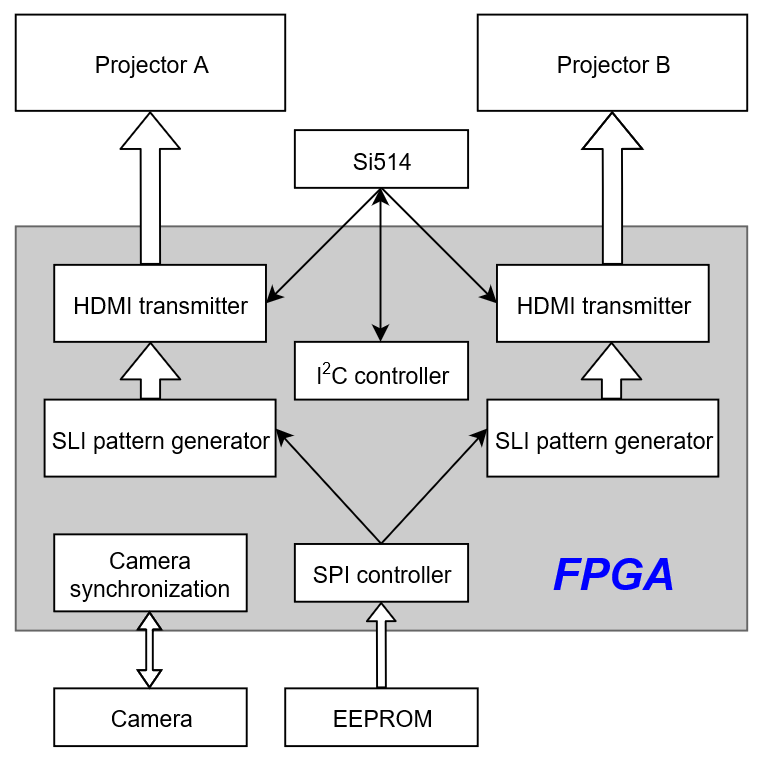
\includegraphics[height=7cm]{sysdg.png}
   %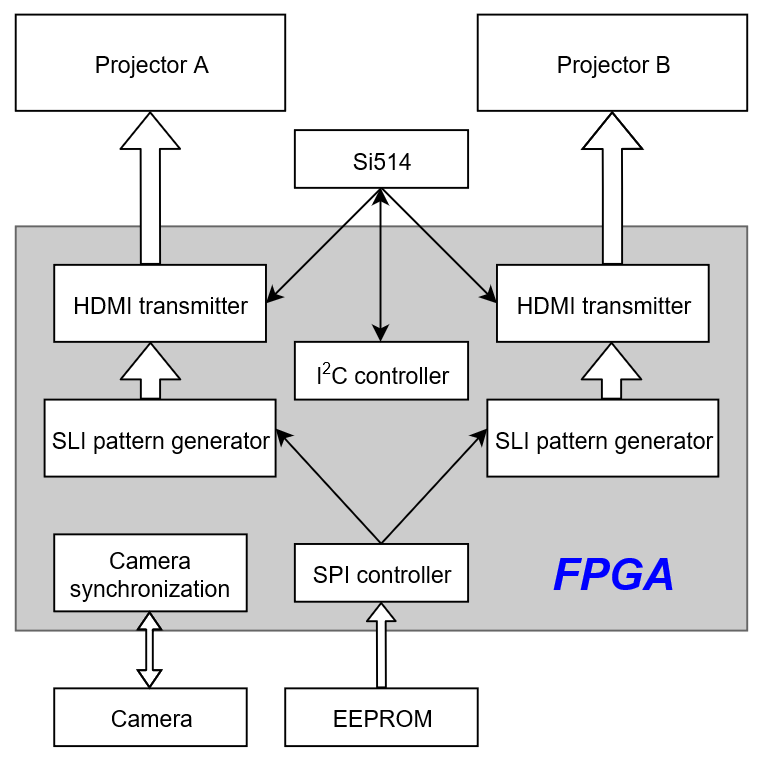
\includegraphics[width=\linewidth]{sysdg.png} 
   \end{tabular}
   \end{center}
   \caption{System diagram}
   \label{Fig:1}
   \end{figure} 

HDMI is the abbreviation of High-Definition Multimedia Interface, it is one of the most popular display interfaces. The newest release, HDMI Version 2.1 supports up to $10K$ video at $120 Hz$. A standard HDMI connector has 19 pins as listed in Table \ref{Tab:1}. Data channel 2, 1, 0 are mainly used to transfer red, green and blue components of the video respectively. The HDMI does not only transfer video data, but also some auxiliary data, for example audio data, packet header. The auxiliary data, video data as well as some control signals are encoded in data channel 2, 1, 0 and then digitally transmitted in serial. In between any two adjacent video periods, one or more data island period and control period are inserted. 

% Please add the following required packages to your document preamble:
% \usepackage[table,xcdraw]{xcolor}
% If you use beamer only pass "xcolor=table" option, i.e. \documentclass[xcolor=table]{beamer}
\begin{table}[!b]
\caption{HDMI pinout}
\label{Tab:1}
\centerline{
\begin{tabular}{|c|l|}
\hline
\rowcolor[HTML]{C0C0C0} 
{\color[HTML]{000000} \textbf{PIN}} & \multicolumn{1}{c|}{\cellcolor[HTML]{C0C0C0}{\color[HTML]{000000} \textbf{DATA}}} \\ \hline
\multicolumn{1}{|l|}{Data2+, Data2 Shield, Data2-} & red pixel component, CTL2, CTL3 and auxiliary data \\ \hline
\multicolumn{1}{|l|}{Data1+, Data1 Shield, Data1-} & green pixel component, CTL0, CTL1 and auxiliary data \\ \hline
\multicolumn{1}{|l|}{Data0+, Data0 Shield, Data0-} & blue pixel component, HSYNC, VSYNC and auxiliary data \\ \hline
\multicolumn{1}{|l|}{Clock+, Clock Shield, Clock-} & pixel clock \\ \hline
SCL, SDA & DDC channel, the source reads the EDID from the sink \\ \hline
CEC & data or commands from remote control \\ \hline
Reserved/HEAC+ & reserved for v1.3 and before, Ethernet and audio since v1.4 \\ \hline
HOT PLUG DETECT/HEAC- & indicate the hot plug or paired with HEAC+ \\ \hline
+5V, Ground & power from external or HDMI source, ground \\ \hline
\end{tabular}\\}
\end{table}

In HDMI, there are six important control signals, HSYNC indicates the beginning and end of a row in a frame of the video, VSYNC indicates the beginning and end of a frame, CTL0~CTL3 indicate the data type of the following data period. The three data channels are transmitted through a differential signaling technology called Transition-Minimized Differential Signaling (TMDS) to reduce the impact of electromagnetic interference and enable high clock skew tolerance. %Another common application of TMDS is in the Digital Visual Interface (DVI).

The 5 volts power signal is provided by the HDMI source or an external source, which after the HDMI sink reads the 5~volts signal, it immediately asserts the pin, Hot Plug Detect. Once the HDMI source detects the presence of a sink by the assertion of the pin Hot Plug Detect, it sends an $I^2C$-based command of a read request to the sink. The pins SCL and SDA compose the display data channel (DDC) via which the Extended Display Identification Data (EDID) is read by the HDMI source from the sink as the response to the read request. The EDID is usually 128 or 256 bytes long, it contains various information related to the features of display system, including but not limited to, manufacturer ID, serial number, week and year of manufacture, screen size, supported timing, etc.

The pin CEC is used to add some advanced functionalities for the HDMI systems. Usually it is a remote control that issues different high-level commands to the devices connected by HDMI cables. CEC stands for Consumer Electronics Control, it is also a one-wire bus protocol, the implementation of CEC is optional, because not all the HDMI devices support this feature. Since HDMI 1.4, the previously reserved pin has become the HDMI Ethernet and Audio Returen Channel (HEAC). While it is in audio return channel mode, only the HEAC+ line is used to transmit audio data; in HDMI Ethernet channel mode, the HEAC+ line pairs up with the HEAC- line as a differential signal to establish a high speed Ethernet communication.

The camera synchronization module controls the timing of the camera trigger signal, it detects the end of the camera's exposure time and makes sure that during the whole camera's exposure time, there is no different pattern projected and every unique phase-shifting fringe pattern is pictured sequentially by the camera. The projector in our SLI system operates at the resolution of $800x600$ and the refresh rate of $120 Hz$. According to the document from VESA \cite{vesa07}, the HDMI timing should be set as Table \ref{Tab:2} lists.

\begin{table}[!b]
\caption{HDMI timing of $800\times 600$ at $120~\mbox{Hz}$}
\label{Tab:2}
\parbox{.45\linewidth}{
\centering
\begin{tabular}{|l|l|}
\hline
\textbf{Pixel Clock} & 73.250MHz \\ \hline
\textbf{Hor. Front Porch} & 48 pixels \\ \hline
\textbf{Hor. Sync Time} & 32 pixels \\ \hline
\textbf{Hor. Back Porch} & 80 pixels \\ \hline
\end{tabular}}
\hfill
\parbox{.45\linewidth}{
\centering
\begin{tabular}{|l|l|}
\hline
\textbf{Ver. Front Porch} & 3 lines \\ \hline
\textbf{Ver. Sync Time} & 4 lines \\ \hline
\textbf{Ver. Back Porch} & 29 lines \\ \hline
\end{tabular}
}\\
\end{table}

To obtain the uncommon 73.25MHz pixel clock, we utilize a programmable oscillator Si514. By configuring the internal registers through $I^2C$ bus, Si514 can generate any frequency from 100kHz to 250MHz with a tuning resolution of 0.026 ppb. Therefore, an $I^2C$ master controller was incorporated into the system. One last module in the system is a lookup table (LUT) that is used to linearize the output of the projector. Ideally, the input digital values of the projector is proportional to the light intensity at the output side of the projector. The light intensity is measured by reading the pixel value of the photo taken by the camera. However, in practice, they are non-linear for most of the times due to some intrinsic characteristics of the projector, e. g. gamma distortion \cite{gamm10}. Applying a LUT to compensate the non-linearity is an effective way to address this problem, as shown in the Figure \ref{Fig:2}, the x-axis represents the 8-bit input digital value of the projector at a certain point of the scene, the y-axis represents the light intensity of the same point that is measured from camera's perspective.

This LUT can be hard-coded into the configuration file of the FPGA, but the drawback is that once the lookup table changes, the FPGA configuration file has to be changed. It is quite inconvenient especially when the system needs to be often applied to a different projector, because generating a new FPGA configuration file requires special software tool and takes more time. We devise a method that the user stores the LUT in an separate EEPROM chip which can be erased and written by any computer via some general serial or USB tools, and the SPI master module in the FPGA reads the EEPROM every time the system  is powered on. With this approach, users can load new LUTs much faster and easier.

\begin{figure}
   \begin{center}
   \begin{tabular}{c}
   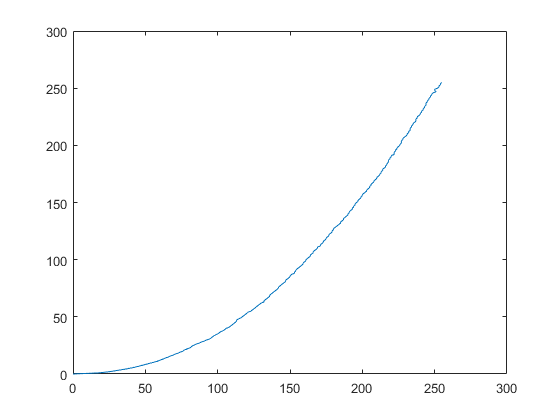
\includegraphics[height=7cm]{wolut.png}
   %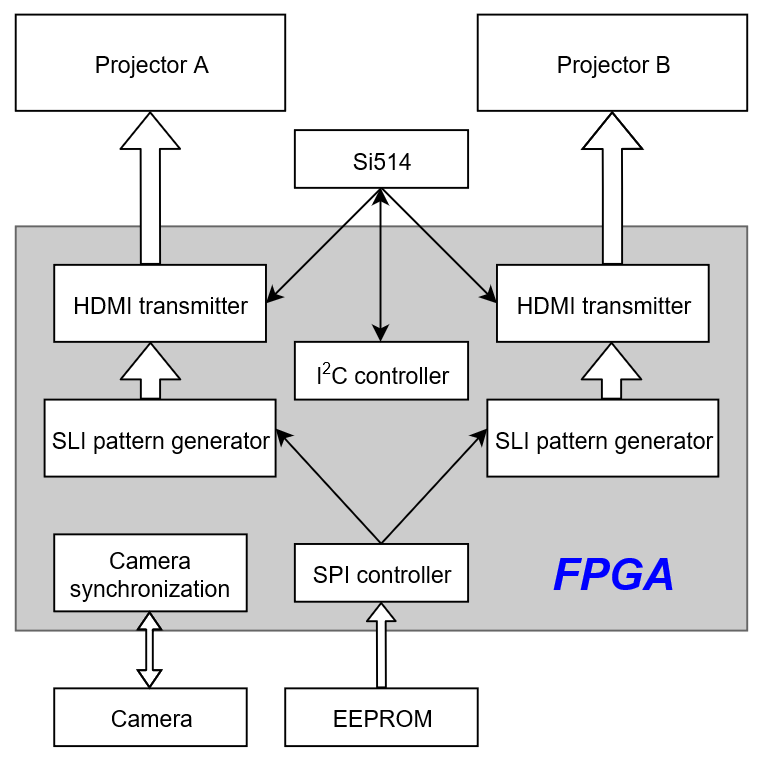
\includegraphics[width=\linewidth]{sysdg.png} 
   \end{tabular}
   \end{center}
   \caption{Non-linearity of the projector Optoma ML750ST}
   \label{Fig:2}
   \end{figure} 


Figure \ref{Fig:3} shows a picture of our tested system.

\begin{figure}
   \begin{center}
   \begin{tabular}{c}
   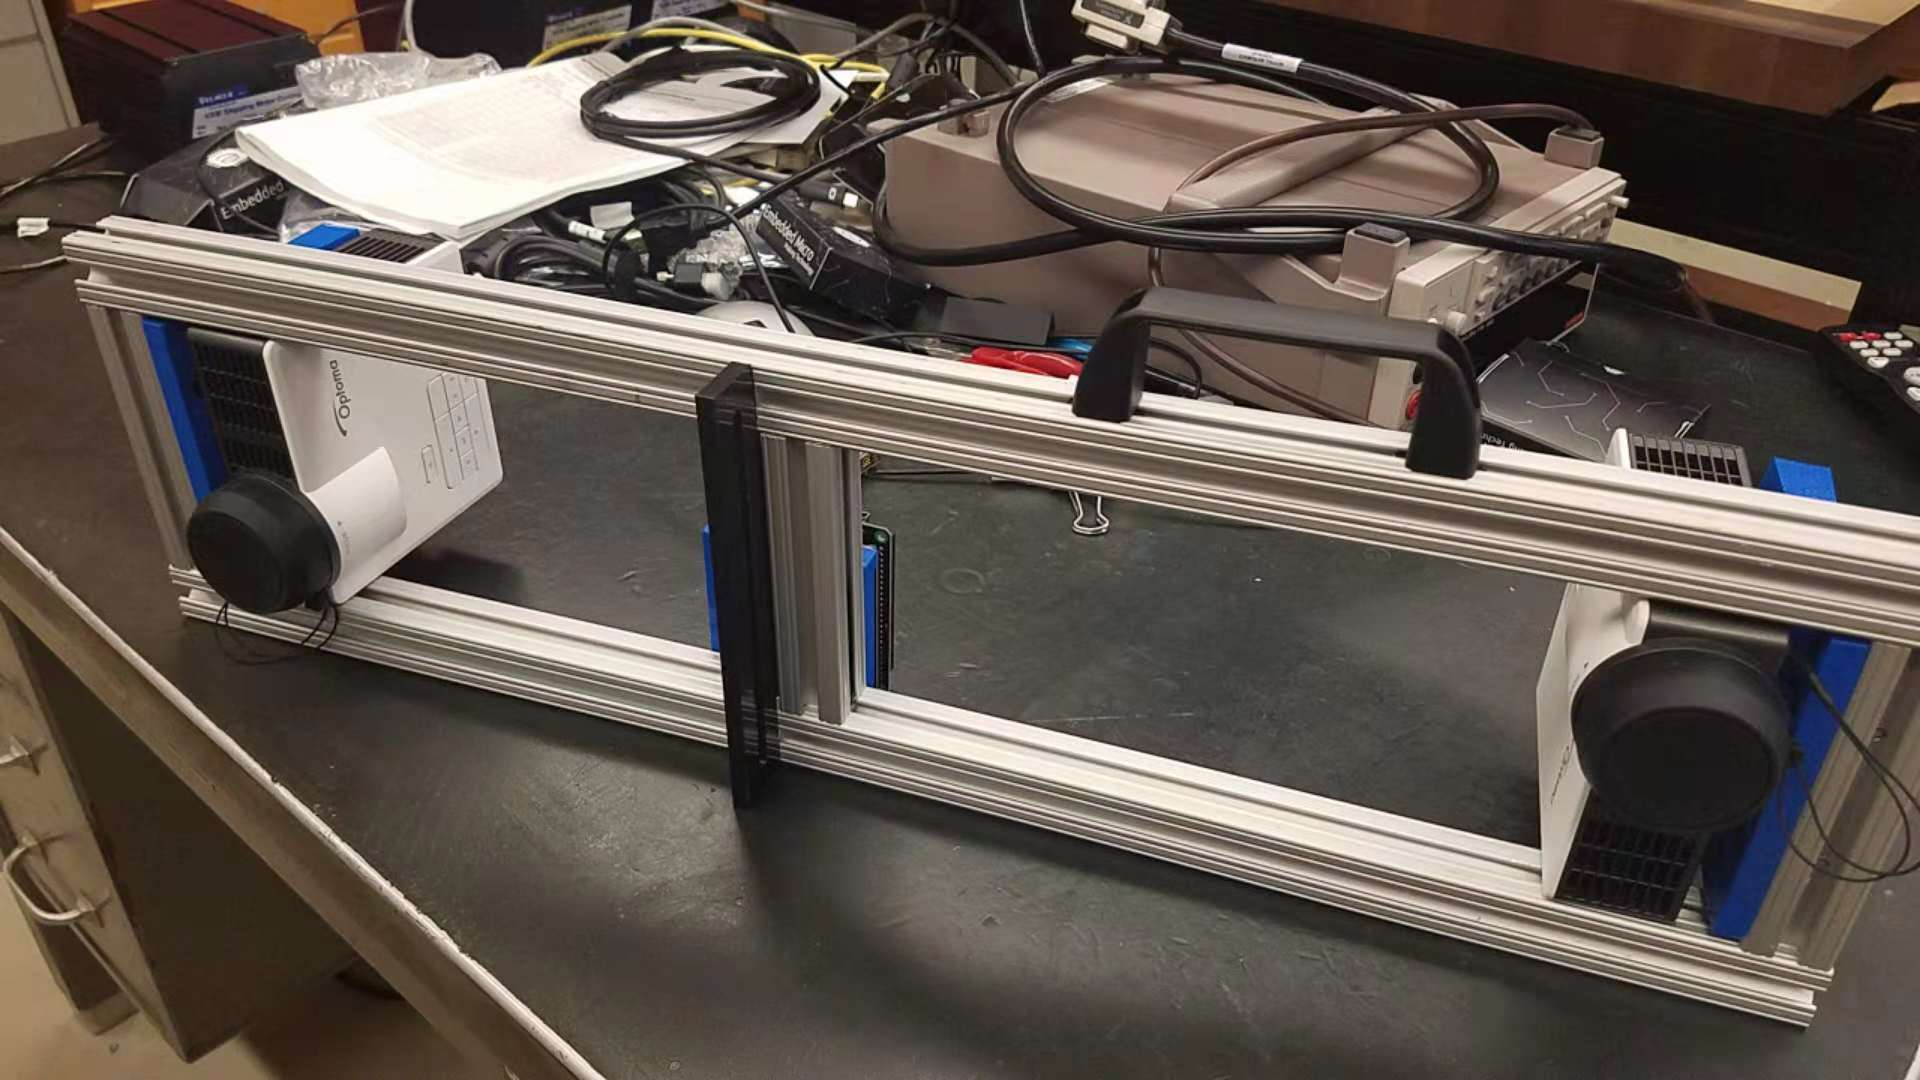
\includegraphics[height=7cm]{dpphoto.jpg}
   %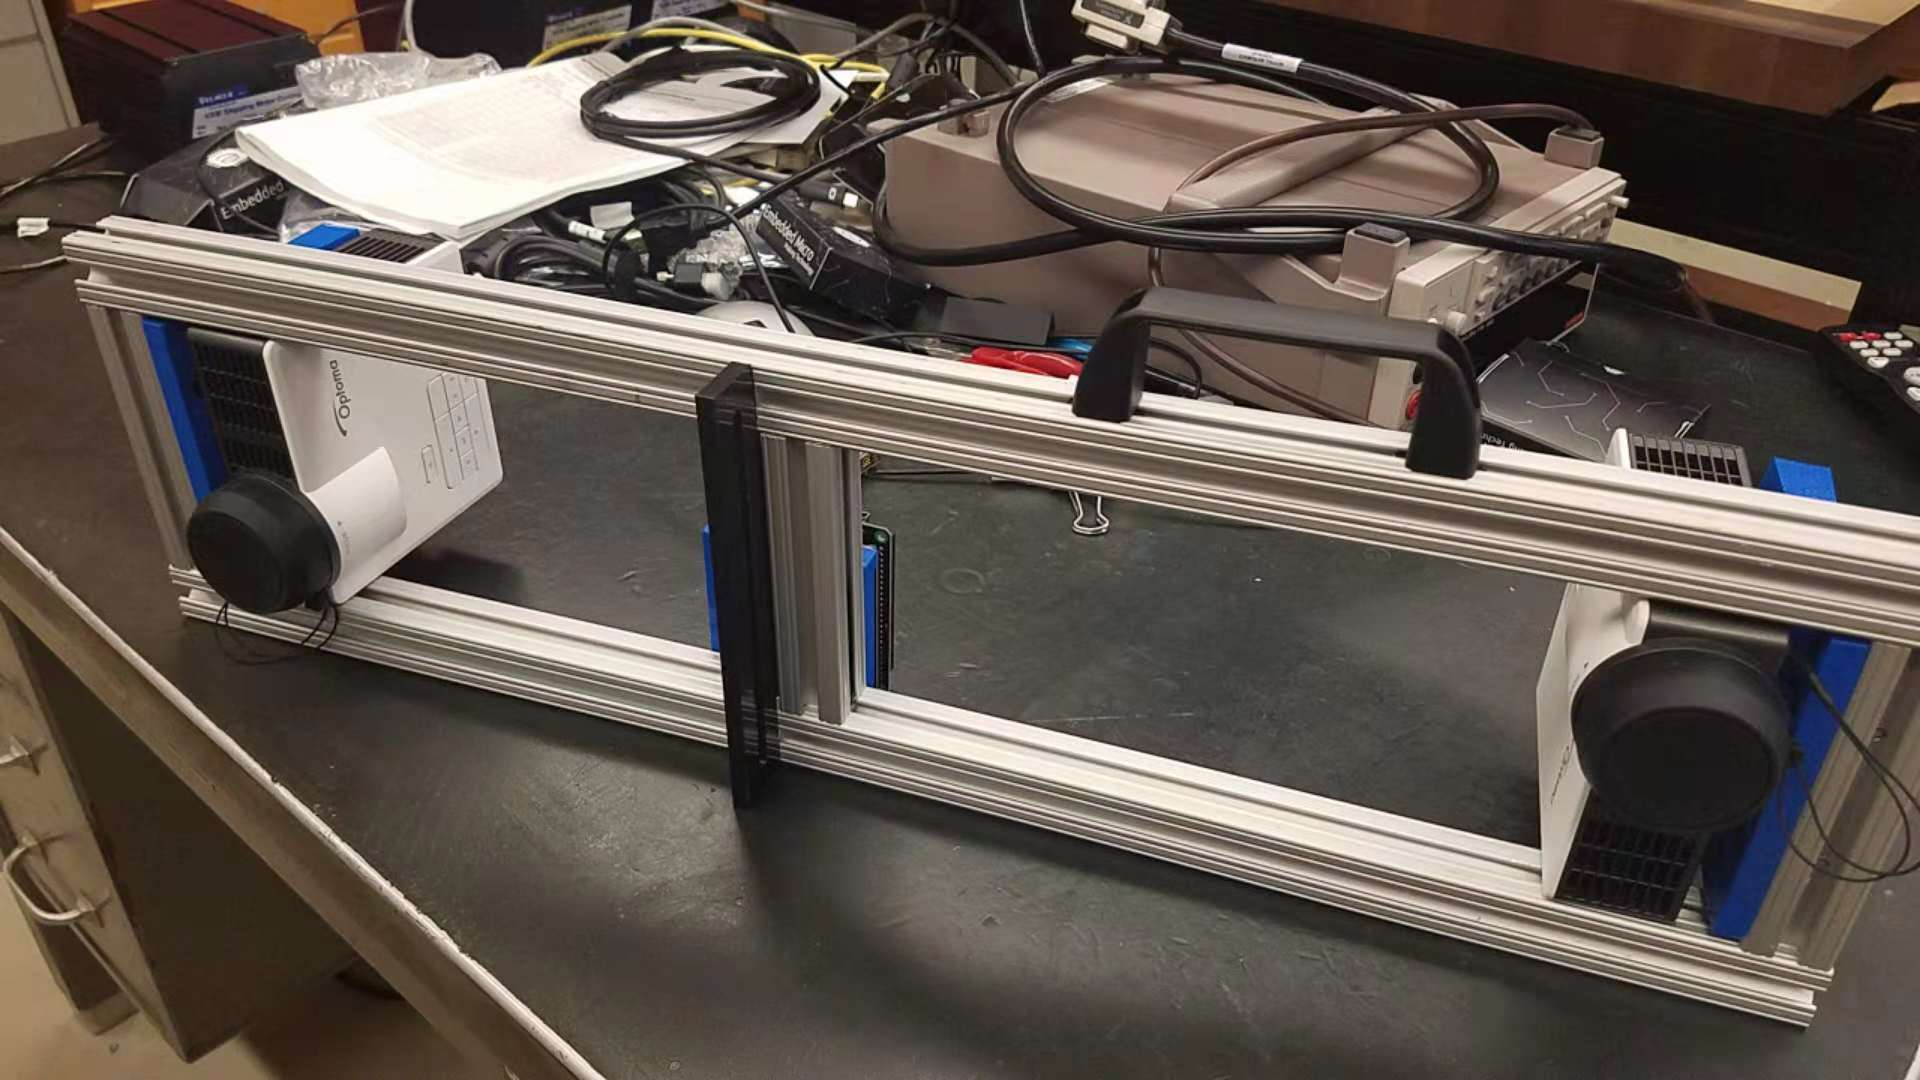
\includegraphics[width=\linewidth]{dpphoto.jpg} 
   \end{tabular}
   \end{center}
   \caption{the dual-projector SLI system}
   \label{Fig:3}
   \end{figure} 


%%%%%%%%%%%%%%%%%%%%%%%%%%%%%%%%%%%%%%%%%%%%%%%%%%%%%%%%%%%%%
%%%%% References %%%%%

\bibliography{report}   %>>>> bibliography data in report.bib
\bibliographystyle{spiebib}   %>>>> makes bibtex use spiebib.bst

\end{document} 
